\chapter{Theory: The Basics}

Over the last decades, quantum chemistry has emerged as a crucial tool for investigating a wide variety of problems in chemistry. This, in combination with the increasing performance and widespread use of computers, has spawned a whole new branch of chemsitry known as \emph{computational chemistry}. The field of computational chemistry uses methods developed in \emph{theoretical chemistry} and incorporates them into efficient programs. Nowaydays, quantum chemical methods are routinely applied to assist in solving problems related to chemical structure, reactivity and spectroscopy. However, one of the main problems in computational chemistry is choosing a suitable level of theory for a given problem - the best choice is always a trade-off between speed and accuracy, and requires intricate knowledge of the methods' theoretical and computational limits. This chapter summarizes the core concepts of quantum chemsitry and introduces the most important methods used in modern computational chemistry. It is by no means complete, and the reader is referred to the original text book resources used by the author for more details (Szabo,Jensen,Helgaker,Schirmer,Norman).

\section{Describing Dynamics in a Molecular System}

In order to describe a molecular system, one needs to decide
\begin{itemize}
\item what the fundamental particles are
\item what forces are governing them
\item what the starting conditions are
\item and what form the dynamical equations take.
\end{itemize}
\noindent The choice of particles dictates what properties the model is ultimately able to describe. For example, force field methods use atoms as the indivisible unit, which is sufficient to describe the molecular structure and dynamics of large molecules such as proteins, but does not provide any information on electron distribution. Using electrons and nuclei as the fundamental particles allows to get a better picture of the electron density and how it reacts to external perturbation, which is important for studies on reactivity and spectroscopic constants. To describe radioactive decay, it is necessary to further divide the nuleus into protons and neutrons. 

Smaller subdivisions lead to a stricter limit on the size of molecules that can be treated. Force field methods may describe the dynamics of molecules with several tens of thousands of atoms, while a finer grained method involving electrons can often only desribe molecules one to two orders of magnitudes smaller depending on the approximantion used.

The mathematical form of the dynamical equations is determined by the size and mass of the particles. They can be divided into four regimes (Figure ...). Atoms are sufficiently heavy and slow that their trajectories can be described using classical (newtonian) mechanics. The time evolution of the positions $\mathbf{r}$ of the atoms in a potential $\mathbf{V}$ can be written as
\begin{equation}
-\frac{\partial \mbf{V}}{\partial t} = m\frac{\partial^2 \mathbf{r}}{\partial t}
\end{equation} 
\noindent which is another form of Newton's second law $\mbf{F} = m\mbf{a}$. The potential $\mbf{V}$ is also treated classicaly as the sum of contributions of particle-particle interactions.

For objects with velocities approaching the speed of light, it is necessary to introduce \emph{relativistic effects}. Mass then becomes a function of velocity
\begin{equation}
m = \frac{m_0}{\sqrt{1-v^2/c^2}}
\end{equation}

Classical newtonian mechanics cannot be applied to very light particles, such as electrons, and quantum effects need to taken into considerations. For non-relativistic velocities, the dynamics are governed by the time-dependent Schrödinger equation:
\begin{equation}
\mathbf{\mbf{H} \Psi(\mbf{r},t) = i \frac{\partial \Psi(\mbf{r},t)}{\partial t}}
\end{equation}
\noindent where $\mbf{H}$ is the Hamiltonian operator which is a sum of the kinetic and potential energy operators
\begin{align}
\mbf{H} = \mbf{T} + \mbf{V} \\
\mbf{T} = -\frac{1}{2m} \nabla^2
\end{align}
\noindent and $\Psi$ is the wavefunction of the system, which is obtained as the solution to the Schrödinger Eqaution, and gives the probability of finding a particle at position $\mbf{r}$ at time $t$. Here, atomic units are assumed.

For electrons moving at relativistic speed, for example in the core orbitals in super-heavy atoms, the Hamiltonian takes a more complex form, and the Schrödinger equation is then known as the $\emph{Dirac}$ equation:
\begin{equation}
\mbf{H}_{Dirac} = \left(c\mbf{\alpha} \mbf{p} + \mbf{\beta}mc^2\right) + \mbf{V}
\end{equation}
Here, only the solutions and aproximations to the non-relativistic Schrödinger equation will be discussed.

\begin{figure}
\centering
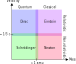
\includegraphics[scale=1.0]{Pics/dyneq}
\caption{Adapted form (ref)}
\end{figure}

\section{The Electronic Schrödinger Equation}

\begin{quote}
  "Where did we get that [Schrödinger's equation] from? It's not possible to derive it from anything you know. It came out of the mind of Schrödinger."
  \begin{flushright}
    \small{--- \textit{Richard Feynman, The Feynman Lectures on Physics}}
  \end{flushright}
\end{quote}

If one is interested in describing the electron distribtion in detail, the Schrödinger Eqaution (SEQ) is the best starting point. There is no formal, rigorous proof for the Schrödinger equation, similar to how Newton's second law cannot really be "derived", more than simply "motivated" by observation. 

As successful as the Schrödinger equation is, finding solutions to it is non-trivial. Different approximations may be applied to the SEQ to solve it more easily, without considerable loss of accuracy. 

\subsection{The Time-Independent Schrödinger Equation}

The potential energy operator is the only time-dependent part of the Hamiltonian:
\begin{equation}
\mbf{H}(\mbf{r},t) = \mbf{T}(\mbf{r}) + \mbf{V}(\mbf{r},t)
\end{equation} 
\noindent For systems where the potential is time-independent, e.g. bound systems without external (electromagnetic) perturbation, the Hamiltonian is time-indepedent as well, which in turn allows to separate space and time variables. It can then be shown that the \emph{time-independent} Schrödinger equation takes the form
\begin{equation}
\mbf{H}\Psi(\mbf{r}) = E \Psi(\mbf{r})
\end{equation}
\noindent where $E$ is the total energy of the system, and the eigenvalue of the wavefunction $\Psi$. The time-depedence is then simply reduced to a phase factor:
\begin{equation}
\Psi(\mbf{r},t) = e^{-iEt} \Psi(\mbf{r})
\end{equation}
\noindent 

\subsection{The Born-Oppenheimer Approximation}

Atomic nuclei are much heavier than electrons ($m_{proton} \approx 1836 m_{electron}$), and move much slower. To a good approximation, the nuclei can be assumed to be stationnary from the point of view of electrons. This is known as the \emph{Born-Oppenheimer approximation}. The total Hamiltonian operator can be written in terms of the kinetic and potential operator of the nuclei ($n$) and electrons ($e$) as
\begin{equation}
\mbf{H}_{tot} = \mbf{T}_n + \mbf{T}_e + \mbf{V}_{ne} + \mbf{V}_{ee} + \mbf{V}_{nn}
\end{equation}
\noindent In the Born-Oppenheimer approximation, the kinetic energy of the nuclei $T_{nn}$ is neglected, and the nucleus-nucleus potential $V_{nn}$ is taken as a constant, which corresponds to neglecting the coupling between electrons and nuclei. This allows a separation of the electronic and nuclar variables. The remaining terms of Equation ... form the electronic Hamiltonian $\mbf{H_{elec}}$. The solutions to the \emph{electronic Schrödinger eqaution}
\begin{equation}
\mbf{H}_{elec} \Psi_{elec}(\mbf{r}_i, \mbf{R}_n ) = E_{elec}(\mbf{R}_n) \Psi_{elec}(\mbf{r}_i, \mbf{R}_n )
\end{equation}
\noindent produce the electronic wavefunction which depends on the (fixed) \emph{position} $\mbf{R}_n$ of the nuclei and no longer on the \emph{momentum} of the nuclei. The total energy
\begin{equation}
E_{tot}(\mbf{R}_n) = E_{elec}(\mbf{R}_n) + E_{nucl}(\mbf{R}_n)
\end{equation} 
\noindent provides a \emph{potential energy surface} (PES) on which the nuclei move. The PES can then be used to solve the nulcear Schrödinger equation to obtain information on vibrational, rotational and translational properties in the molecular system.

From this point onward, the subscript $elec$ is dropped, and only the electronic Schrödinger Equation is considered.

\section{Solutions to the Electronic Schrödinger Equation}

\subsection{Slater Determinants}

It is first important to consider the wave function of the single electrons. In single-atom systems, these functions take the form of "atomic orbitals" (AOs). Correspondingly, "molecular orbitals" (MOs) are defined as the single electron wave functions in a molecular system. These spatial orbital functions form the basis of the total electronic wave function.  

The Hamiltonian in ... only depends on the spatial coordinates. However, to fully describe an electron, one also needs to consider spin. This is done by introducing two orthonormal spin functions $\alpha(\omega)$ and $\beta(\omega)$ corresponding to spin-up ($\uparrow$) and spin-down ($\downarrow$), with the spin-coordinate $\omega$. For one spatial molecular orbital, this gives two possible \emph{spin-orbitals}
\begin{equation}
\phi(\mathbf{x}) = \left\lbrace\begin{matrix}
\varphi(\mathbf{r}) \alpha(\omega) \\
\varphi(\mathbf{r}) \beta(\omega)
\end{matrix} \right.
\end{equation}
\noindent where $\varphi$ are the \emph{spatial orbitals}, and $\mathbf{x}$ are the combined spatial and spin coordinates. The spin orbitals therefore depend on four variables.

To a first approximation, one may consider a molecular system to consist of $N$ \emph{non-interacting}, independent electrons. The Hamiltonian is then written as a sum of one-particle Hamiltonians 
\begin{equation}
\mathbf{H} = \sum_i^N \mathbf{h}_i 
\end{equation}
\noindent Electron correlation may then be included in some average way by using \emph{effective} one-electron Hamiltonians, which is the basic working idea of the \emph{Hartree} method. The solution to the SEQ can then be expressed as a product of the one electron wave functions
\begin{equation}
\Psi^{HP}(\mbf{x}_1,\mbf{x}_2,...,\mbf{x}_N) = \phi(\mbf{x}_1) \phi(\mbf{x}_2) ... \phi(\mbf{x}_N)
\end{equation}
\noindent which is also known as \emph{Hartree product}. 

However, the Hartree product does not take into account the \emph{indistinguishability} of electrons. In what is known as the antisymmetry principle, which is a generilization of the Pauli exclusion principle, the wave function needs to fulfill 
\begin{equation}
\Psi(\mbf{x}_1,\mbf{x}_2) = - \Psi(\mbf{x}_2,\mbf{x}_1) 
\end{equation}
\noindent upon exchange of any two electrons in the system. This is most easily achived by using \emph{Slater determinants} (SD). For a molecular system consisting of $N$ electrons distributed over $N$ spin orbitals $\phi_i$, the SD takes the form
\begin{equation}
\Psi_{SD}(\mbfx_1, \mbfx_2, \ldots, \mbfx_N) = \frac{1}{\sqrt{N!}}
\begin{vmatrix}
\phi_I(\mbfx_1) & \phi_J(\mbfx_1) & \ldots & \phi_P(\mbfx_1) \\
\phi_I(\mbfx_2) & \phi_J(\mbfx_2) & \ldots & \phi_P(\mbfx_2) \\
\vdots & \vdots & \ddots & \vdots \\
\phi_I(\mbfx_N) & \phi_J(\mbfx_N) & \ldots & \phi_P(\mbfx_N) \\
\end{vmatrix}
\end{equation}
\noindent Or, using the diagonal of the SD as a short-hand notation
\begin{equation}
\Psi_{SD}(\mbfx_1, \mbfx_2, \ldots, \mbfx_N) = \ket{\phi_I(\mbfx_1) , \phi_J(\mbfx_1), \ldots, \phi_K(\mbfx_1)}
\end{equation}

\subsection{The Fock Space}

A more generalized representation of the space of the antisymmetrized electron wave functions can be achieved by introducing the concept of occupation number (ON) vectors in the context of second quantization (Annex). In a system with $M$ possible states (in this case spin molecular orbitals), the ON vectors take the form
\begin{equation}
\ket{\mbf{k}} = \ket{k_1, k_2, \ldots, k_M} = 
\left\lbrace
\begin{matrix}
1 \textit{if $\phi_P$ occupied} \\
0  \textit{if $\phi_P$ occupied}
\end{matrix}
\right.
\end{equation}
\noindent The occupation number is 1 if $\phi_P$ is present in the SD, and 0 if not. Together, all possible ON vectors in Equation ... form an orthonormal abstract vector space, known as Fock space. The Fock space formed by $N$ electrons distributed over $M$ orbitals is denoted as $F(M,N)$ with total dimension equal to the binomial coefficient $\begin{bmatrix} M \\ N \end{bmatrix}$. The sum of the occupation numbers in the ON vectors gives the total number of electrons
\begin{equation}
N = \sum_i^M k_i
\end{equation}
\noindent The special fock space $F(0,M)$ contains a single vector known as the vacuum state with
\begin{align}
\ket{vac} = \ket{0_1, 0_2, \ldots, 0_M} \\
\bra{vac}\ket{vac} = 1
\end{align}
\noindent The ON vectors in $F(M,N)$ can be alternatively expressed in terms of the vaccum state from $F(M,0)$ using creation operators
\begin{equation}
\ket{\mbf{k}} = \left[ \prod_{P=1}^M (a\pdg_P)^{k_P} \right] \ket{vac}
\end{equation}
\noindent In second quantization, the antisymmetry principle of the wavefunction is guaranteed by the commutator relationship of the annihilation and creation operators $a_P$ and $a\pdg_P$ which act on the ON vectors.

\subsection{Exact Solution and Standard Models}

The simplest approach to solving the electronic SEQ is by approximating the exact wave function $\Psi$ using a single Slater determinant where the electrons occupy the lowest lying molecular orbitals. The Hartree-Fock method is an example of a \emph{single-determinant method} and finds \emph{the} single best Slater determinant for $\ket{\Psi}$. In Fock space, the best possible determinant is represented by the ON vector where the $N$ lowest lying orbitals are occupied. 

As will be discussed in more detail later, a single-determinant treatment of the electronic wavefunction is insufficient to fully capture \emph{electron correlation}. The electron correlation energy is formerly defined as the difference between the Hartree-Fock energy and the \emph{exact} energy of $\ket{Psi}$
\begin{equation}
E_{correlation} = E_{HF} - E_{exact}
\end{equation}
\noindent although the Hartree-Fock wave function does include correlation effects to some degree. In a more general sense, electron correlation is a broad term for any interactions between electrons that make their movement depend on each other, or \emph{correlate} with each other (cf Section ...). 

In order to improve on the HF approximation, it is important to add additional Slater determinats. These SDs can be generated from the HF reference wave function by replacing the occupied MOs $\phi_I$ in a reference Slater determinant ... by one or multiple orbitals $\phi_A$ which were previously unoccupied. This effectively corresponds to exciting one or more electrons from their occupied molecular orbitals $I,J,..$ to unoccupied, or $virtual$ orbitals $A,B,..$ (Figure ...). These excited Slater determinants can be classified by the number of electrons they excite and are often referred to as singles, doubles, triples and so on.
\begin{align*}
\ket{S} &= a\pdg_A a_I \ket{HF} \\
\ket{D} &= a\pdg_A a_I a\pdg_B a_J \ket{HF} \\
\ket{T} &= a\pdg_A a_I a\pdg_B a_J a\pdg_C a_K \ket{HF} \\
\ldots &
\end{align*}
\noindent Alternatively, singles states are known as 1-particle-1-hole (1p-1h or simply p-h) states, doubles as 2-particle-2-hole (2p-2h) and so on, due to the excitation operators effectively creating \emph{holes} in the reference determinant and adding \emph{particles} in higher lying orbitals instead. 

The exact solution to the electronic Schrödinger equation is then given by the sum of the Hartree Fock wave function and all possible ON vectors in $F(M,N)$
\begin{equation}
\ket{\Psi} = c_0 \ket{HF} + \sum^{{{M}\choose{N}}-1}_{i=1} c_i  \ket{i} 
\end{equation}  
\noindent Equation ... offers a systematic approach to improve on the Hartree Fock method, by increasing (1) the number of Sater determinats and (2) the basis set size $M$, and gives rise to a hierarchy of methods. Correlated electronic structure methods mainly differ by how they determine the expansion coefficients $c$. For all but the smallest systems, the full $F(M,N)$ cannot be used in calculations due to the total number of ON vectors which increases binomially with ${M}\choose{N}$, and hence the number of coefficients to be determined. In practice, the Fock space is \emph{truncated} to some degree.

\begin{figure}
\centering
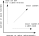
\includegraphics[scale=2.0]{Pics/standardmodel}
\caption{Standard model}
\end{figure}

\emph{Multi-determinant} methods like configuration interaction (CI) or coupled cluster (CC) use the Hartree Fock wave function as the reference from which they generate singles, doubles, triples ... SDs  as in Eqaution .... By truncating at different excitation levels, one gets a hierarchy of CI/CC methods which recover different amounts of correlation energy (e.g. CIS, CISD, CISDT ...). Multi-determinant methods are mainly suited to recover dynamic correlation (cf. ...).

For systems with strong static correlation, additionally, a multi-reference approach is needed. Here, the excited SDs are generated from multiple reference states rather than only from HF. Methods include multireference CI (MRCI) and multireference CC (MRCC). The reference states are traditionally obtained from multiconfigurational self-consistent-field methods (MCSCF) like the complete active space SCF (CASSCF) or restrcited active space SCF (RASSCF). MCSCF is a combination of HF and CI, which both optimizes the HF molecular coefficients and the CI expansion coeffcients. Multi-reference methods methods mainly recover \emph{static correlation} (cf. Section ...). (Note: in limit, both static and dynamic recovered. No strict division between them)

A summary of all \emph{ab-initio} standard models is given in Figure ...

Different Route: Moller plesset

\subsection{The Variational Method}

The time-independent Schrödinger equation takes the form of an eigenvalue problem
\begin{equation}
\mbf{H} \ket{\Psi_i} = E_i \ket{\Psi_i} \qquad i=0,1,2,...\infty
\label{eq:SEQINFTY}
\end{equation}
\noindent where the infinite set of exact solutions $\ket{\Psi_i}$ with eigenvalues $E_i$ forms an orthonormal basis
\begin{equation}
\bra{\Psi_i}\ket{\Psi_j} = \delta_{ij}
\end{equation} 
\noindent A trial wavefunction can be expanded in the basis of exact solutions with coefficients $c$ as
\begin{equation}
\ket{\tPsi} = \sum_i a_i \ket{\Psi_i}
\label{eq:trialwave}
\end{equation}
\noindent The \emph{variation principle} states that the expectation value of the Hamiltonian of an approximate wave function of the form \ref{eq:trialwave} is an upper bound to the exact ground state energy. This statement can be expressed as
\begin{equation}
\frac{\bra{\tPsi}\mbf{H}\ket{\tPsi}}{\vphantom{\widetilde{\Psi}} \bra{\tPsi}\ket{\tPsi}} \geq E_0
\end{equation}
\noindent The equality only holds when $\ket{\tPsi}$ is equal to the exact solution $\ket{\Psi_0}$. One can recast the eigenvalue problem \ref{eq:SEQINFTY} as a variational optimization problem where the energy is a functional of a trial wavefunction
\begin{equation}
E[\tPsi] = \frac{\bra{\tPsi}\mbf{H}\ket{\tPsi}}{\vphantom{\widetilde{\Psi}} \bra{\tPsi}\ket{\tPsi}}
\end{equation}
\noindent The saddle points of the energy functional then correspond to the exact solutions of the Schrödinger equation. The variational approach to the SEQ provides a powerful tool to solve a wide variety of problems in electronic structure theory.

The trial wave function depends on a set of coefficients $c$, and hence the energy functional will also depend on these coefficients. In general, determining the coefficients which minimize the functional is very difficult. However, a more simple approach of the variational method can be obtained by using a linear ansatz where the trial function is expanded in a fixed N-dimensional set of orthonormal basis functions $\ket{\phi}$
\begin{equation}
\ket{\tPsi} = \sum^N_i c_i \ket{\phi_i}
\end{equation}
By using Lagrange's method of undetermined multipliers
\begin{align}
\mathcal{L}(\mbf{c},E) &= \bra{\tPsi}\mbf{H}\ket{\tPsi} - E(\bra{\tPsi}\ket{\tPsi} - 1) \\
\frac{\partial \mathcal{L}}{\partial \mathcal{\mbf{c}}} &= 0
\end{align}
\noindent it is possible to show that the variational problem corresponds to solving the eigenvalue problem involving the Hamiltonian matrix $\mbf{H}$:
\begin{equation}
\mbf{H}\mbf{c}_n = E_n \mbf{c_n}
\end{equation}
\noindent Or, in a more general form
\begin{equation}
\mbf{H}\mbf{C} = \mbf{C}\mbf{E}
\end{equation}
\noindent Here, $\mbf{C}$ is a $N$ by $N$ coeffcient matrix containing $N$ column coefficient vectors $\mbf{c}_n$ ($n$ = $0...N$) which describe $N$ possible solutions for the trial wave function $\ket{\tPsi}$. $\mbf{E}$ is a diagonal matrix containing the eigenvalues $E_n$. This approach of finding approximate solutions to the eigenvalue problem \ref{eq:SEQINFTY} is known as the \emph{linear variational method}. 

\section{Hartree Fock}

The Hartree Fock method is central to electronic structure method. It is computationally inexpensive, and is still routinely used in qualititative studies of large molecules, even if it does not accurately account for electron correlation. It also serves as the starting point for correlated methods. Only a few computational methods actually bypass the solution to the Hartree Fock equations, firmly cementing its place in quantum chemsitry.

\subsection{The Hartree Fock Equations}

Recall the structure of the electronic Hamiltonian
\begin{equation}
\mbf{H} = \mbf{T}_e + \mbf{V}_{ne} + \mbf{V}_{ee} + \mbf{V}_{nn}
\end{equation}
\noindent with
\begin{align}
\mbf{T}_e &= -\sum_i^N \frac{1}{2} \nabla_i^2 \qquad \textrm{kinetic energy of electrons} \\
\mbf{V}_{ne} &= -\sum_a^{N_{nuc}} \sum_i^N \frac{Z_a}{\mid\mbf{R}_a - \mbf{r}_i\mid} \qquad \textrm{nuclei-electron repulsion} \\
\mbf{V}_{ee} &= \frac{1}{2} \sum^N_i \sum^N_{j \neq i} \frac{1}{\mid \mbf{r}_i - \mbf{r}_j\mid} \qquad \textrm{electron-electron repulsion} \\
\mbf{V}_{nn} &= \frac{1}{2}\sum_a^{N_{nuc}} \sum_{b \neq a}^{N_{nuc}} \frac{Z_a Z_b}{\mid \mbf{R}_a - \mbf{R}_b \mid} \qquad \textrm{nuclei-nuclei repulsion} 
\end{align}
\noindent In Hartree-Fock theory, the electrons are treated as independent particles. One can therefore ignore the coupling between electrons in the $\mbf{V}_{ee}$ and express the Hamiltonian as a sum of an effective one-electron operator $\mbf{f}$, also known as the \emph{Fock} operator, of the form
\begin{align}
\mbf{H} &= \sum_i \mbf{f}_i =  \sum_i \mbf{h}_i + \frac{1}{2} \sum_i \sum_{j \neq i} \mbf{g}_ij  \\
\mbf{h}_i &= -\frac{1}{2}\nabla_i^2 - \sum_a^{N_{nuc}} \frac{Z_a}{\mid \mbf{R}_a - \mbf{r}_i |} \\
\mbf{g}_{ij} &= \frac{1}{\mid \mbf{r}_i - \mbf{r}_j \mid}
\end{align}
\noindent The one-electron operator $\mbf{h}$, also known as the \emph{core} Hamiltonian describes the movement of the electrons in the field of the nuclei. The two-electron operator $\mbf{g}_{ij}$ gives the average potential (or "field") experienced by electron $i$ due to the presence of all the other electrons $j$. For this reason, Hartree-Fock is also known the \emph{mean-field} approximation. In second quantization, the fock operator takes the form
\begin{equation}
\mbf{f} = \sum^{M}_{PQ} h_{PQ} a\pdg_P a_Q + \frac{1}{2} \sum^{M}_{PQRS} g_{PQRS} a\pdg_P a\pdg_R a_S a_Q
\label{eq:FOCK2Q}
\end{equation}
\noindent with the matrix elements of the one and two electron operators given by
\begin{align}
h_{PQ} &= \bra{\phi_P} \mbf{h} \ket{\phi_Q} = \int \phi_P^*(\mbf{x}) h(\mbf{x}) \phi_Q(\mbf{x}) d\mbf{x} \\
g_{PQRS} &= \bra{PQ}{RS} = \int\int \phi_P^*(\mbf{x}_1) \phi^*_R(\mbf{x}_2) g(\mbf{x}_1,\mbf{x}_2) \phi_Q(\mbf{x}_1) \phi_S(\mbf{x}_2) d\mbf{x}_1 d\mbf{x}_2
\end{align} 
\noindent The elements $g_{PQRS}$ are known as the 2-electron repulsion integrals. Calculating the expectation values for the fock operator in \ref{eq:FOCK2Q} using second quantization gives (ref):
\begin{equation}
\begin{split}
f_{PQ} &= \bra{\phi_P} \mbf{f} \ket{\phi_Q} \\
	&= h_{PQ} + \sum_{I}^N \frac{1}{2} (g_{PQII} - g_{PIIQ}) \\
	&= h_{PQ} + \frac{1}{2} (J_{PQ} - K_{PQ})
\end{split}
\end{equation} 
\noindent The symmetric matrix with entries $f_{PQ}$ is also known as the \emph{Fock matrix}. $\mbf{J}$ is the \emph{coulomb matrix} and describes electron correlation due to the coulomb potential (coulomb correlation), and $\mbf{K}$ is the exchange matrix describing the electron correlation which arises due to the Pauli exclusion principle (Fermi correlation). The exchange contributions have no classical counterpart and arise purely from quantum mechanical considerations.

In the special basis where the Fock matrix is diagonal
\begin{equation}
f_{PQ} = \delta_{PQ} \eps_P 
\end{equation}
\noindent the one-electron eigenfunctions of the Fock operator 
\begin{equation}
\mbf{f} \ket{\phi_P} = \eps_P \ket{\phi_P} 
\label{eq:HFEQ}
\end{equation} 
\noindent are known as the \emph{canonical molecular spin orbitals}, and the eigenvalues are the \emph{molecular orbital energies}. Solving the \emph{Hartree-Fock equation} \ref{eq:HFEQ} gives the MOs which form the basis of Hartree-Fock wavefunction. It should be stressed that the total electronic Hartree Fock energy is not the sum of the individual MO energies, but is given by the expectation value of the Hamiltonian 
\begin{equation}
E_{HF} = \bra{HF}\mbf{H}\ket{HF} = \sum_{I}^{N} h_{II} + \frac{1}{2} \sum_{I}^{N} \left( J_{II} - K_{II} \right)   
\end{equation}
\noindent where the sum runs over the \emph{occupied} orbitals $I$. For $N$ electrons distributed over $M$ MOs, there are $N$ occupied orbitals with $\eps_I < 0$ and $M-N$ virtual orbitals with $\eps_A > 0$. 

\subsection{The Basis Set Approximation}

Up until this point, the electronic wavefunction was constructed from Slater determinants of molecular spin orbitals. Virtually all applications use a basis set expansion to express the unknown MOs in terms of known functions, conventially called \emph{atomic orbitals}. Any type of function can be used, e.g. exponentials, gaussians, polynomials or plane waves. Exponentials and gaussians are best suited to describe bound systems. The molecular orbitals are then expressed as a \emph{linear combination of atomic orbitals} (LCAO)
\begin{equation}
\ket{\phi_i} = \sum_i^{M_{basis}} c_{i\mu} \chi_{\mu} 
\end{equation}
\noindent The basis set approximation is \emph{exact} for an infinite number of basis functions. For more details, see ...  

\subsection{Working Equations for Restricted and Unrestricted Hartree-Fock}

For reasons of efficient implementation, it is useful to separate out different electron spin components. The Fock matrix has four spin blocks: $F_{\alpha\alpha}$, $F_{\alpha\beta}$, $F_{\beta\alpha}$ and $F_{\beta\beta}$. The Fock matrix in the canonical basis is diagonal, and therefore only the diagonal blocks  $F_{\alpha\alpha}$ and $F_{\beta\beta}$ are important. Introducing the notation $\olI$ for MOs with spin $\sigma'$, and $I$ with opposite spin $\sigma$, the matrix elements of a spin block are given by
\begin{equation}
\begin{split}
f_{PQ}^{\sigma} &= h_{PQ}^{\sigma} + \frac{1}{2} \left\lbrace \sum^{N_{\sigma}}_{PQ}\sum^{N_{\sigma}}_{I} \cn{PQ}{II} - \cn{PI}{QI}  - \sum^{N_{\sigma}}_{PQ}\sum^{N_{\sigma'}}_{I} \cn{PQ}{\olJ\olJ} - \cn{P\olJ}{Q\olJ} \right\rbrace \\
&= h_{PQ}^{\sigma} + \sum^{N_{\sigma}}_{PQ} J^{\sigma}_{PQ} - K^{\sigma}_{PQ} + J^{\sigma'}_{PQ} - K^{\sigma'}_{PQ}
\end{split}
\end{equation}
\noindent The opposite spin block $f_{PQ}^{\sigma'}$ is obtained by substituting indices with a bar by indices without a bar and vice-versa. Spin separation yields two coupled sets of equations for alpha and beta MOs
\begin{equation}
\begin{split}
\mbf{f}^{\alpha} \ket{\phi^{\alpha}_I} &= \eps^{\alpha}_I \ket{\phi^{\alpha}_I} \\
\mbf{f}^{\beta} \ket{\phi^{\beta}_I} &= \eps^{\beta}_I \ket{\phi^{\beta}_I} 
\end{split}
\label{eq:UHF}
\end{equation} 
\noindent These are known as the unrestricted Hartree-Fock equations (UHF). For closed-shell molecules with equal number of alpha and beta elecrons, the spatial part of the MOs is the same for both spins. The expression for the Fock matrix then further simplifies to 
\begin{equation}
f_{ij} = h_{ij} + 2J_{ij} - K_{ij} 
\end{equation}
\begin{equation}
\mbf{f} \ket{\phi_i} = \eps_i \ket{\phi_i}
\label{eq:RHF}
\end{equation}
\noindent The equations in \ref{eq:RHF} are known as the restricted Hartree-Fock (RHF) equations. 

\noindent Using the linear variatonal method explained in the previous section for the MO trial functions expressed as a linear combination of $N_{bas}$ AO basis functions, the eigenvalue problem for RHF can be recast in matrix form as
\begin{align}
\mbf{F} \mbf{C} &= \mbf{C} \mbf{E} 
\end{align}
\noindent with the MO coefficient matrix $\mbf{C}$ and the Fock matrix $\mbf{F}$ in the AO basis given by
\begin{align}
F_{\mu\nu} &= H^{core}_{\mu\nu} + \sum_{\lambda\sigma}^{N_{basis}} \left(2 \cn{\mu\nu}{\sigma\lambda} P_{\lambda\sigma} - \cn{\mu\sigma}{\nu\lambda} P_{\lambda\sigma} \right) \\
&= H^{core}_{\mu\nu} + 2 J_{\mu\nu} - K_{\mu\nu} 
\end{align}
\noindent The symmetric matrix $\mbf{P}$ is the so-called atomic orbital density matrix (DM) of the form
\begin{equation}
P_{\mu\nu} = \sum_i^{N_{occ}} C_{\mu i} C_{\nu i} 
\end{equation}
\noindent A similar expressions is found for UHF
\begin{equation}
\begin{split}
F_{\mu\nu}^{\sigma} &= H^{core}_{\mu\nu} + \sum_{\lambda\sigma}^{N_{basis}} \left( \cn{\mu\nu}{\sigma\lambda} P^{T}_{\lambda\sigma} - \cn{\mu\sigma}{\nu\lambda} P^{\sigma}_{\lambda\sigma} \right) \\
P^T_{\mu\nu} &= P^{\sigma}_{\mu\nu} + P^{\sigma'}_{\mu\nu} 
\end{split}
\end{equation}
\noindent where the AO spin-density matrices $\mbf{P}^{\sigma}$ are defined as the product of the corresponding coefficient matrices with spin $\sigma$.  

\subsection{The Self-Consistent Field Method}

In general, the atomic orbitals are not orthogonal. Defining the overlap matrix $\mbf{S}$ with entries 
\begin{equation}
S_{\mu\nu} = \int \chi_{\mu}^*(\mbf{r}) \chi_{\nu}^*(\mbf{r}) d\mbf{r}
\end{equation}
\noindent where $S_{\mu\mu} = 1$, the eigenvalue problem for RHF takes the more general form
\begin{equation}
\mbf{F} \mbf{C} = \mbf{SC} \mbf{E}
\label{eq:RHALL}
\end{equation}
\noindent The equations in \ref{eq:RHALL} are known as the \emph{Roothan equations}. In the unrestricted case, they are called the \emph{Pople-Nesbet equations}:
\begin{align}
\mbf{F}^{\alpha} \mbf{C}^{\alpha} &= \mbf{SC}^{\alpha} \mbf{E}^{\alpha} \\
\mbf{F}^{\beta} \mbf{C}^{\beta} = \mbf{SC}^{\beta} \mbf{E}^{\beta}
\end{align}  

%In the HF approximation, the molecular system is treated as $N$ independent electrons where the Hamiltonian operator is expressed as a sum of $N$ effective Hamiltonians
%
%% give form of electronic hamiltonian
%% collect them in 1elec components and 2elec components, second quantization
%% fock operator, mean field
%% evaluation of fock matrix elements / energy
%% restricted form.
%
%\subsection{SCF}
%
%\subsection{What does HF miss}
%
%\begin{equation}
%\mbf{H} = \sum^N_i \mbf{f}(i) 
%\end{equation}
%\noindent where $\mbf{f}$ is also known the \emph{Fock} operator, of the form
%\begin{equation}
%\mbf{f} &= \mbf{h} + \mbf{v}^{HF}
%\label{eq:FOCKOPERATOR}
%\end{equation}
%\noindent Here, $\mbf{h}$ is a one-electron operator, also known as the core Hamiltonian, which sums the kinetic and nuclei-electron repulsion part:
%\begin{equation}
%\mbf{h} = -\frac{1}{2} \nabla^2 - \sum^{M_{nuc}}_{A=1} \frac{Z_A}{r_{A}} 
%\end{equation} 
%\noindent where $Z$ is the nuclear charge, and $r_{A}$ is the nucleus-electron distance. The two-electron operator $\mbf{v}^{HF}$ in the Fock operator describes the average potential (or "field") experienced by electron $i$ due to the presence of all the other electrons. For this reason, Hartree-Fock was originally known as the \emph{mean-field} approximation. In second qunatization, the Fock operator can be written as
%\begin{equation}
%\mbf{f} = \sum_{PQ} h_{PQ} a\pdg_P a_Q + \frac{1}{2} \sum_{PQRS} g_{PQRS} a\pdg_P a\pdg_R a_S a_Q  
%\end{equation}



\section{Electron Correlation}

\section{Post-Hartree Fock Ground State}

\subsection{Configuration Interaction}

\subsection{Perturbation Theory}

\subsection{Coupled Cluster}

\section{Post-Hartree Fock Excited State}

\subsection{Coupled Cluster Linear Repsonse}

\subsection{Equation-of-Motion Coupled Cluster}

\subsection{Algebraic Diagrammatic Construction}
